% Supporting information for the campaign paper (#277). Build: make si
\documentclass[11pt]{article}
\usepackage[margin=1in]{geometry}
\usepackage[T1]{fontenc}
\usepackage{lmodern}
\usepackage{amsmath}
\usepackage{graphicx}
\usepackage{booktabs}
\usepackage{xcolor}
\usepackage{textcomp}
\usepackage[hidelinks]{hyperref}
\usepackage[numbers]{natbib}
\renewcommand{\thetable}{S\arabic{table}}
\renewcommand{\thefigure}{S\arabic{figure}}
\renewcommand{\thesection}{S\arabic{section}}
\newcommand{\placeholder}[1]{\textcolor{red!75!black}{[#1]}}
\newcommand{\note}[1]{\textcolor{blue!70!black}{\textsf{\footnotesize [Note: #1]}}}
\newcommand{\AlSi}{AlSi10Mg}
\newcommand{\Scal}{Scalmalloy}
% Generated by scripts/make_figures.py. Do not edit by hand.
\newcommand{\InhouseYS}{228}
\newcommand{\InhouseYSsd}{13}
\newcommand{\InhouseYShw}{21}
\newcommand{\InhouseUTS}{376}
\newcommand{\InhouseUTSsd}{10}
\newcommand{\InhouseEL}{4.5}
\newcommand{\InhouseELsd}{0.5}
\newcommand{\InhouseN}{4}
\newcommand{\NAlRuns}{\placeholder{N runs}}
\newcommand{\NCompositions}{\placeholder{N compositions}}
\newcommand{\BAlSinir}{\placeholder{B}}
\newcommand{\BAlSicost}{\placeholder{B}}
\newcommand{\BScalnir}{\placeholder{B}}
\newcommand{\BScalcost}{\placeholder{B}}


\title{Supporting Information\\[4pt]\large \placeholder{Title as in the main text}}
\author{\placeholder{Authors}}
\date{\placeholder{Date}}

\begin{document}
\maketitle

\note{Every section below is tied to a row of ../figure-plan.csv (S1--S10), with its data file and due date. The three tables in Section S3 are generated by ../scripts/make\_figures.py from data/ and are current; the rest are placeholders.}

\section{Atomizer runs used in this work}
\placeholder{A table with one row per Al run in the campaign (date, composition, charge mass, melt set point, hold, plate, booster, amplitude, pour pressure, O\textsubscript{2}, outcome, powder mass below 250 and 63~\textmu m), including failed runs, generated from atomizer-runs/runs.csv. Due 12 Feb 2027 (owner: Gage).}

\section{CALPHAD settings and the full ranked list}
\placeholder{Databases and versions, Scheil settings (step, fast diffusers, stop at $f_s$), the criteria and how they were combined, the element bounds, and every screened composition with its scores. Due 29 Jan 2027 (owner: Xavier).}

\section{Critical-mineral burden: inputs and sensitivity}
Table~\ref{tab:elements} lists the per-element inputs of the burden metrics in the main text: whether the element is on the final 2025 U.S.\ List of Critical Minerals~\cite{fr2025}, its U.S.\ net import reliance in 2025, and its 2025 price~\cite{usgs2026}. Where USGS gives only a bound (for example, silicon above 50\%), the burden is reported as the interval the bound allows. Prices are on mixed bases (U.S.\ spot for Al, Si, Mg, Cu; ex-works China or FOB for Sc, Zr and the rare earths), and manganese metal has no 2025 price in USGS sources, so the 2023 value is used.

\begin{table}[htbp]
  \centering\scriptsize
  \caption{Per-element inputs of the burden metrics (data/element-criticality.csv).}
  \label{tab:elements}
  \resizebox{\textwidth}{!}{\begin{tabular}{@{}lllrl@{}}
\toprule
Element & On 2025 list & U.S.\ net import reliance, 2025 (\%) & Price (USD\,kg$^{-1}$) & Price basis \\
\midrule
Al & yes & 60 (metal); bauxite $>$75 & 3.97 & ingot, U.S. spot, 180 cents/lb (converted) \\
Si & yes & $>$50 (metal and ferrosilicon; metal alone $>$50) & 2.87 & silicon metal, 130 cents/lb Si, Jan-Oct mean (converted) \\
Mg & yes & $>$75 & 7.05 & metal, U.S. spot Western, \$3.20/lb (converted) \\
Mn & yes & 100 & 3.48 & electrolytic metal, 157.79 cents/lb (converted); 2023 value, Minerals Yearbook, as MCS 2026 gives only ore \\
Cr & yes & 79 & 13.01 & metal, \$5.90/lb gross weight (converted) \\
Zr & yes & $<$25 (ores and concentrates); net exporter of Zr metal & 22.00 & sponge, ex-works China \\
Sc & yes & 100 & 5200.00 & metal, ex-works China (oxide \$640/kg; Al-2Sc ingot \$30/kg of master alloy) \\
Fe & no & net exporter (iron ore) & -- & not on the list; left out of B\_cost \\
Cu & yes & 57 & 10.80 & cathode, U.S., 490 cents/lb (converted) \\
Ni & yes & 41 & 15.00 & LME cash, \$15,000/t \\
Ce & yes & 67 (all rare-earth compounds and metals) & 2.10 & CeO2 $\geq$99.5\% FOB \$1.71/kg, per kg of contained Ce (oxide basis, not metal) \\
Er & yes & 100 (heavy rare earths) & 52.60 & Er2O3 $\geq$99.5\% FOB \$46/kg, per kg of contained Er (oxide basis, not metal) \\
Ti & yes & 100 (sponge) & 12.00 & sponge, landed import value \\
Ag & yes & 77 & 1222.00 & \$38/troy oz (converted) \\
V & yes & 41 & 19.75 & V2O5 \$5.02/lb, per kg of contained V (oxide basis) \\
B & yes & net exporter & -- & no element price (borates only) \\
Zn & yes & not collected & -- & not collected \\
\bottomrule
\end{tabular}
}
\end{table}

\placeholder{Sensitivity: the ranking of the benchmarks, the seeds and the campaign alloys under $B_\mathrm{NIR}$ (low, midpoint, high), $B_\mathrm{cost}$ (scandium priced as metal and as Al--2Sc master alloy), and scandium content.} Counting aluminum itself at its 60\% import reliance (left out of the main metric because it is the base of every alloy) adds a large, nearly equal term to every alloy (aluminum is 89--98~wt\% of them) and squeezes the differences: \AlSi{} then scores \BAlSinirallo--\BAlSiniralhi~wt\%, \Scal{} \BScalnirallo--\BScalniralhi~wt\% and seed S1 \BSonenirallo--\BSoneniralhi~wt\%, so S1 falls inside \Scal's interval. On the current inputs without aluminum, \AlSi{} scores \BAlSinirlo--\BAlSinirhi~wt\% and Scalmalloy \BScalnirlo--\BScalnirhi~wt\% on $B_\mathrm{NIR}$, and \BAlSicost{} and \BScalcost~USD\,kg\textsuperscript{-1} on $B_\mathrm{cost}$.

\begin{figure}[htbp]
  \centering
  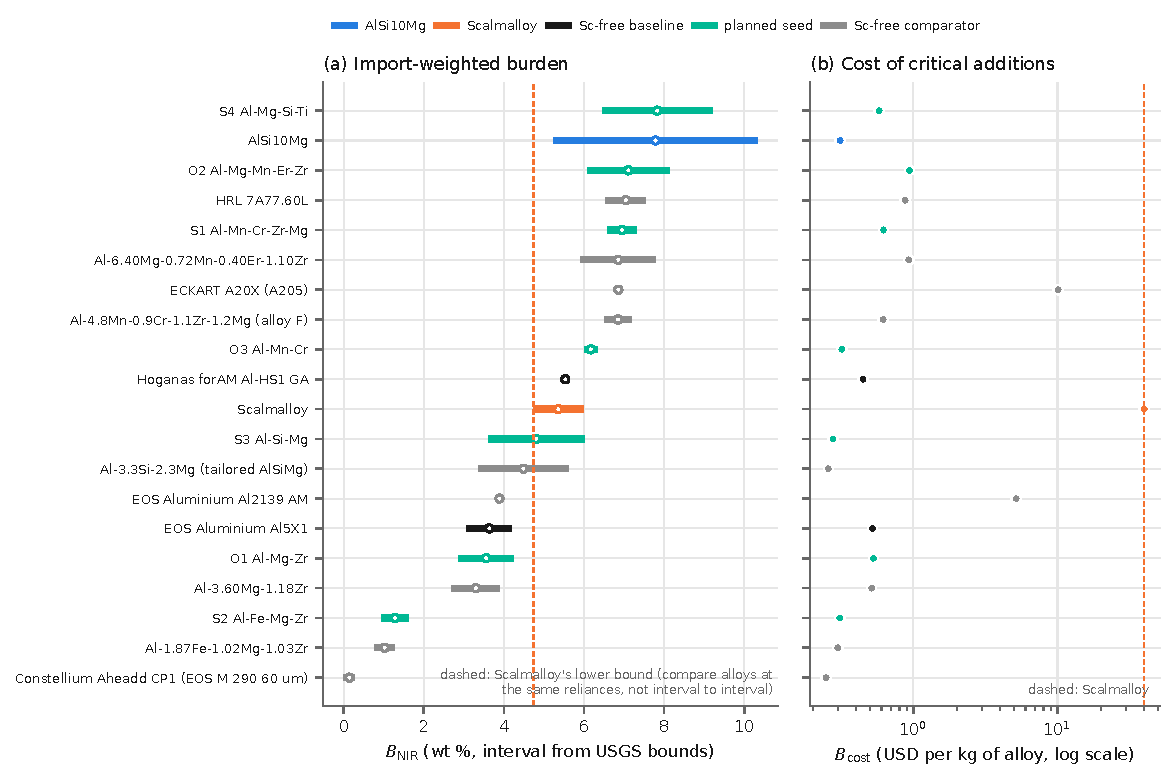
\includegraphics[width=\textwidth]{figures/figS1-burden-sensitivity.pdf}
  \caption{Critical-mineral burden of every alloy in this work, two ways. (a) Import-weighted burden $B_\mathrm{NIR}$: the bar is the interval allowed by the import reliances USGS gives only as bounds, the dot its midpoint; dashed, the lower end of \Scal's interval. (b) Cost of the critical alloying additions per kilogram of alloy, scandium priced as metal (log scale); dashed, \Scal. The two metrics rank the alloys differently: \Scal is mid-table on (a) and far above every other alloy on (b). The A20X cost leaves out boron, which has no element price.}
  \label{fig:burden}
\end{figure}

\subsection*{Scandium-free comparators}
Table~\ref{tab:literature} lists the scandium-free alloys drawn in Fig.~1 of the main text, with their burden on the same inputs.
\begin{table}[htbp]
  \centering\scriptsize
  \caption{Scandium-free LPBF aluminum alloys from vendor datasheets and papers, at the condition with the highest yield strength listed, with their burden. Values were transcribed by an earlier survey of this project (26 Nov 2026) and checked against each source on 27 Nov 2026; two rows could not be verified because the full texts were not accessible (data/literature-alloys.csv, read\_by column). Nominal compositions use the midpoints of published ranges.}
  \label{tab:literature}
  \resizebox{\textwidth}{!}{\begin{tabular}{@{}llrrrrl@{}}
\toprule
Alloy & Condition (highest yield listed) & YS (MPa) & EL (\%) & $B_\mathrm{NIR}$ (wt\%) & $B_\mathrm{cost}$ (USD\,kg$^{-1}$) & Source \\
\midrule
Hoganas forAM Al-HS1 & direct aged 375 C 4 h & 370 & 12.0 & 5.4--5.6 & 0.45 & \cite{ds_hoganas} \\
EOS / Constellium Al5X1 & direct aged 400 C 6 h (ASTM E8) & 385 & 14.5 & 3.1--4.2 & 0.52 & \cite{ds_al5x1} \\
Constellium Aheadd CP1 (EOS M 290 60 um) & heat treated 400 C 4 h & 300 & 10.0 & 0.0--0.3 & 0.25 & \cite{ds_cp1} \\
ECKART A20X (A205) & T7 & 440 & 13.0 & 6.8--6.9 & -- & \cite{ds_a20x} \\
HRL 7A77.60L & HIP + heat treatment & 585 & 14.0 & 6.5--7.5 & 0.88 & \cite{ds_7a77} \\
Al-4.8Mn-0.9Cr-1.1Zr-1.2Mg (alloy F) & aged 375 C 8 h & 500 & 5.0 & 6.5--7.2 & 0.62 & \cite{almncrzr2024} \\
Al-6.40Mg-0.72Mn-0.40Er-1.10Zr & aged 375 C 10 h & 440 & 15.5 & 5.9--7.8 & 0.93 & \cite{almgmnerzr2022} \\
Al-1.87Fe-1.02Mg-1.03Zr & aged 400 C 4 h & 376 & 11.1 & 0.8--1.3 & 0.30 & \cite{alfezr2025} \\
Al-3.3Si-2.3Mg (tailored AlSiMg) & as built (Concept Laser M2) & 417 & 10.1 & 3.4--5.6 & 0.26 & \cite{alsimg2020} \\
EOS Aluminium Al2139 AM & T4 (490 C 45 min, water quench, 3 days RT) & 460 & 6.0 & 3.8--3.9 & 5.16 & \cite{ds_al2139} \\
Al-3.60Mg-1.18Zr & peak aged (about 8 h at 400 C, inferred) & 353 & 18.6 & 2.7--3.9 & 0.51 & \cite{croteau2018} \\
\bottomrule
\end{tabular}
}
\end{table}

\subsection*{Comparing burdens at the same import reliances}
USGS gives the import reliance of silicon, magnesium and zirconium only as bounds, so each alloy's $B_\mathrm{NIR}$ is an interval. The bound is the same unknown for every alloy, so two alloys are compared under the same reliances: $B_\mathrm{NIR}(a) - B_\mathrm{NIR}(b) = \sum_i (w_{a,i} - w_{b,i})\,\mathrm{NIR}_i/100$ is linear in each reliance, and its range over all allowed values is reached at the bounds, taking for each element the high bound where alloy $a$ has more of it and the low bound where it has less. Table~\ref{tab:paired} gives that range against \Scal for the benchmarks, the baselines and the planned seeds; ``below'' means below at every allowed reliance, ``depends'' that the sign changes within the bounds. It also gives $B_\mathrm{mass}$, the plain mass of the alloying elements on the 2025 list, and $B_\mathrm{cost}$. Comparing interval with interval, as an earlier draft did (an alloy's whole interval below the lower end of \Scal's), sets one alloy at one reliance against another at a different one; it gives the same verdicts here but is stricter than the question needs.

\begin{table}[htbp]
  \centering\scriptsize
  \caption{$B_\mathrm{NIR}$ against \Scal{} with both alloys under the same import reliances, nominal compositions (data/alloys.csv). The baselines' rows use their vendors' typical values or range midpoints until the outside laboratory measures their lots; With Si and Ti at zero, Al5X1's Mg--Zr--Mn range spans $B_\mathrm{NIR}$ 2.0--5.7~wt\% and stays below \Scal{} at every corner; with Si and Ti at their allowed 1.0~wt\% it reaches 7.65~wt\% and would not, so the lot's measured composition decides.}
  \label{tab:paired}
  \resizebox{\textwidth}{!}{\begin{tabular}{@{}llllrr@{}}
\toprule
Alloy & $B_\mathrm{NIR}$ (wt\%) & $B_\mathrm{NIR} - B_\mathrm{NIR}^\mathrm{Scal}$, same reliances (wt\%) & vs \Scal & $B_\mathrm{mass}$ (wt\%) & $B_\mathrm{cost}$ (USD\,kg$^{-1}$) \\
\midrule
AlSi10Mg & 5.2--10.3 & $-0.66$ to ${+}5.51$ & depends & 10.32 & 0.31 \\
Scalmalloy & 4.7--6.0 & 0 & -- & 6.21 & 39.93 \\
EOS Aluminium Al5X1 & 3.1--4.2 & $-2.01$ to $-1.45$ & below & 5.10 & 0.52 \\
H\"ogan\"as forAM Al-HS1 GA & 5.4--5.6 & $-0.48$ to ${+}0.82$ & depends & 6.40 & 0.45 \\
S1 Al-Mn-Cr-Zr-Mg & 6.6--7.3 & ${+}0.97$ to ${+}2.21$ & above & 8.33 & 0.62 \\
S2 Al-Fe-Mg-Zr & 0.9--1.6 & $-4.71$ to $-3.44$ & below & 2.40 & 0.31 \\
S3 Al-Si-Mg & 3.6--6.0 & $-1.74$ to ${+}0.64$ & depends & 6.00 & 0.28 \\
S4 Al-Mg-Si-Ti & 6.5--9.2 & ${+}1.64$ to ${+}3.29$ & above & 9.20 & 0.58 \\
O1 Al-Mg-Zr & 2.9--4.2 & $-2.14$ to $-1.47$ & below & 5.14 & 0.53 \\
O2 Al-Mg-Mn-Er-Zr & 6.1--8.1 & ${+}1.35$ to ${+}2.14$ & above & 8.95 & 0.94 \\
O3 Al-Mn-Cr & 6.0--6.3 & ${+}0.16$ to ${+}1.47$ & above & 6.50 & 0.32 \\
\bottomrule
\end{tabular}
}
\end{table}

\section{Powders}
\placeholder{Size distributions (D10, D50, D90 and the fraction below 63~\textmu m), shape descriptors, SEM of every lot, EDS acquisition settings (kV, process time, standards), oxygen. Due 12 Feb 2027 (owner: Ronnie).}

\section{Print parameters and build layouts}
\placeholder{Machine, plate, preheat, gas and O\textsubscript{2}, laser power, scan speed, hatch, layer, scan strategy, and photos of each build plate. The April 2026 Utah build's laser parameters are not recorded in the project records and must be obtained from the facility. Due 12 Feb 2027 (owner: Carl).}

\section{Tensile specimens and curves}
\placeholder{Specimen drawing (ASTM E8/E8M sub-size flat), every stress--strain curve including invalid tests, and the yield-strength fit window. The five April 2026 \AlSi{} curves exist (test 4 broke in the grip). Due 15 Feb 2027 (owner: Carl).}

\section{Corrosion set-up validation}
\placeholder{A reference measurement on the CubXL/EZstat-Pro set-up against a standard procedure, before any alloy is tested. Due 15 Jan 2027 (owners: Ben and Jarrett).}

\section{Provenance records}
\placeholder{One page per finalist lot: charge, atomizer settings and video, sieving, storage humidity, print, and every measurement, each with the file that backs it. Due 15 Feb 2027 (owner: Gage).}

\section{Pre-registration}
\placeholder{The comparators and the procedure every alloy follows, the floor rule (``stronger than \AlSi''), the rule for expanding the scandium-free front, the on-par rule, the burden metric and its threshold, and the optimizer settings, with the commit that froze them before the first optimizer round. Due Tue 1 Dec 2026, before the screen ranks any campaign composition and before the seeds are picked at G1 on 4 Dec (owner: Sterling).} A draft is in ../preregistration.md.
The optimizer settings to freeze include the model (Bayesian optimization over function networks~\cite{astudillo2021,buathong2024}, or a single Gaussian-process surrogate), the acquisition function, the batch size, the inputs and the stopping rule.

\section{Commercial powders}
\placeholder{For AlSi10Mg, Al5X1, Al-HS1 and \Scal{}: vendor, lot, the lot certificate's chemistry, oxygen and particle size, the outside laboratory's composition, the power--speed grid and each powder's densest point, build layouts, and the in-house tensile results against each vendor's datasheet with the on-par ratio. Due 12 Feb 2027 (owners: Gage for the orders, Carl for the prints and tests). Sourcing is in ../baselines.md; nothing is ordered yet.}

\bibliographystyle{unsrtnat}
\bibliography{references}
\end{document}
